\documentclass[10pt,twocolumn,a4paper]{article}
\usepackage[margin=1.8cm]{geometry}
\usepackage{booktabs,graphicx,subcaption,siunitx,hyperref,microtype,xcolor}
\usepackage{caption}
\captionsetup{font=small,labelfont=bf}

\title{\textbf{Partitioned Hash Join with Duplicates}\\\large A Distributed MPI Study}
\author{Gabriele Marsili \\ SPM a.y.\ 2025/26}
\date{}

\begin{document}
\maketitle
\thispagestyle{empty}

%---------------------------------------------------------------
\section{Introduction}
%---------------------------------------------------------------
This report describes the distributed implementation of the
partitioned hash join developed throughout the previous modules.
The algorithm is unchanged: $R$ and $S$ are partitioned through a
common key-mapping function and a local join is performed
independently on each partition. The aim of this module is to study
how communication costs interact with local computation when memory
bandwidth and memory capacity are spread across multiple cluster
nodes, and to compare the resulting performance with the
shared-memory variants of Modules~2 and~3.

Two implementations are presented. They share the same algorithmic
skeleton and the same generator scheme as the previous modules: a
pure MPI version that exchanges partitions via
\texttt{MPI\_Alltoallv}, and a hybrid MPI+OpenMP version in which
\emph{every} per-rank phase is parallelised with OpenMP, so that a
single rank can drive all the cores of a node. All experiments were
carried out on the SPM cluster (8 compute nodes, dual-socket Intel
Xeon E5-2640~v2, 32 logical CPUs and \SI{128}{GB} of RAM per node,
Open MPI~5.0.3).

%---------------------------------------------------------------
\section{Distributed Algorithm}
%---------------------------------------------------------------

\subsection{Partitioning and Rank Assignment}
The mapping function from Modules~1--3 is unchanged. A 64-bit key
$k$ is folded to 32~bits and multiplied by the Fibonacci constant,
$p=((k_{\text{lo}}\oplus k_{\text{hi}})\cdot\varphi_{32})\gg(32-\log_2
P)$. Each partition is assigned to one of the $R$ MPI ranks by
$\text{dest}(p)=p\bmod R$ with local index $\ell=p\,\text{div}\,R$
in $[0,P/R)$. The constraint $P\bmod R=0$ keeps the number of
partitions per rank exactly balanced.

\subsection{Pipeline}
Each rank generates only its slice of $R$ and $S$ using
\texttt{splitmix64} skip-ahead so the concatenation of the local
slices equals the sequential generator output byte-for-byte. The
distributed pipeline has eight measured phases:
\emph{histogram\_local}, \emph{scatter\_local} (in dest-major order
so each rank's send buffer is naturally contiguous per destination),
\emph{comm\_sizes} (\texttt{MPI\_Alltoall} of the per-rank counts),
\emph{comm\_payload} (\texttt{MPI\_Alltoallv} of the records),
\emph{histogram\_post} and \emph{scatter\_post} (local re-layout of
the received buffer so the M3 build/probe kernel can be reused
unchanged), \emph{join\_local}, and the final
\texttt{MPI\_Allreduce} of the three aggregates
$(\textit{join\_count},\textit{ck}_1,\textit{ck}_2)$. Each interval
is preceded by an \texttt{MPI\_Barrier} so the rank-local time
reflects the actual critical path; the reduction takes the maximum
across ranks so the breakdown shows the slowest path per phase.

\subsection{Choice of the Redistribution Primitive}
\texttt{MPI\_Alltoallv} was chosen as the canonical primitive for
total-exchange of partitioned data (lez.~25). A non-blocking
alternative based on \texttt{MPI\_Isend/Irecv} was considered: it
gives more control over communication--computation overlap, but the
records sent by every rank to every other rank carry no associative
structure that would justify it, and the breakdown measurements of
\S\ref{sec:breakdown} confirm that the collective implementation
already saturates the network bandwidth on the cluster. A small
\texttt{MPI\_Alltoall} of the per-rank counts precedes each payload
exchange so the receive buffers can be sized exactly.

\subsection{Hybrid MPI+OpenMP}
The hybrid implementation uses one MPI rank per node and
\texttt{OMP\_NUM\_THREADS} equal to the number of logical CPUs.
Every local phase is OpenMP-parallel: \emph{histogram\_local} and
\emph{histogram\_post} use per-thread private histograms merged at
the end, \emph{scatter\_local} and \emph{scatter\_post} reuse those
per-thread histograms to compute per-thread offsets and then write
into the output buffer with static scheduling, and \emph{join\_local}
runs a \texttt{parallel for} with \texttt{schedule(dynamic)} and a
sum reduction. The dynamic schedule on the join mirrors M3's loop
variant under skewed workloads (lez.~14): partition cardinalities
vary and a static split would stall the last threads on the
largest partitions. MPI is initialised with
\texttt{MPI\_THREAD\_FUNNELED} since only the main thread enters
MPI.

%---------------------------------------------------------------
\section{Correctness}
%---------------------------------------------------------------
Three levels of verification were applied. For tiny inputs
($N_R, N_S\le 500$) rank~0 regenerates the full relations and
compares the global $(\textit{join\_count},\textit{ck}_1,
\textit{ck}_2)$ to an $O(N^2)$ naive join. For larger uniform
inputs the same triple is compared to the sequential baseline of
Module~3 across rank counts $R\in\{1,2,4,8\}$ on the laptop and
\{32,64,128\} ranks on the cluster. For skewed inputs the
sequential M3 binary does not accept the skew flags, so the
distributed runs are cross-checked against a single-rank MPI run
using the same parameters. All 36 local cases and all 18 cluster
cases passed; the validation logs are stored in
\texttt{results/validation\_local.log} and
\texttt{results/cluster/validation\_cluster.log}.

%---------------------------------------------------------------
\section{Experimental Setup}
%---------------------------------------------------------------
Strong-scaling, weak-scaling and breakdown runs use $P=256$
partitions, seed $42$ and $\textit{max\_key}=N_R/2$, with five
repetitions per cell and the median time reported. Strong scaling
fixes the global input at $N_R=\SI{50}{M}$ and $N_S=\SI{100}{M}$
records; weak scaling holds the per-rank workload constant at
$N_R/R=\SI{2}{M}$ records (with $N_S/R=\SI{4}{M}$). Pure MPI uses
one rank per logical CPU (32 ranks per node); the hybrid uses one
rank per node with \texttt{OMP\_NUM\_THREADS=32},
\texttt{OMP\_PROC\_BIND=close} and \texttt{OMP\_PLACES=cores}.
The sequential baseline used for speedup is the Module~3
sequential binary, recompiled with \texttt{-march=ivybridge} (the
compute-node ISA, which does not support the AVX2 produced by
\texttt{-march=native} on the Haswell login node) and timed on a
dedicated compute node. The reference time is
$t_{\text{seq}}=\SI{4.52}{s}$ for $N_R=\SI{50}{M}$,
$N_S=\SI{100}{M}$.

%---------------------------------------------------------------
\section{Strong Scaling}
%---------------------------------------------------------------
Figure~\ref{fig:strong} reports the speedup as a function of node
count. The hybrid variant is the clear winner from two nodes
upwards on both workloads. On the uniform dataset the hybrid
speedup grows monotonically from $2.8\times$ at one node to
$12.2\times$ at eight, crossing the ideal $N$-node line because
the per-node cost is dominated by collective communication that
does not grow as fast as the rank count. Pure MPI reaches
$7.7\times$ at two nodes (64 ranks) and $7.1\times$ at eight (256
ranks), but at four nodes (128 ranks) it collapses to $3.1\times$.
The collapse is not measurement noise in the strict sense, but it
is bimodal across the five repetitions: the minimum is \SI{0.68}{s}
(in line with the two-node extrapolation), the median is
\SI{1.48}{s} and four of five runs sit in the slow mode. We
interpret this as Open MPI's Alltoallv algorithm selection at 128
ranks: in the slow mode the collective hits a routing pattern that
the cluster fabric handles poorly, and the choice is not under our
control without injecting MCA tuning parameters. The fact that
both the \SI{0.68}{s} fast mode and the eight-node \SI{0.63}{s}
runs are stable shows that the bandwidth is there; the median is
honest about how often that bandwidth is realised in practice.

Under the skewed dataset the curves separate further. Pure MPI
degrades monotonically from $4.4\times$ at one node to $2.8\times$
at eight: every additional rank adds entries to the
\texttt{Alltoallv} fan-out, but the hot partitions concentrate on
a small number of receivers, so the collective waits on the
slowest ranks. The hybrid version still grows, from $2.9\times$
to $5.1\times$; with at most eight participants the fan-out stays
small and the work per rank is large enough that load imbalance
dominates rather than communication latency.

\begin{figure}[t]
  \centering
  
\includegraphics[width=\linewidth]{fig_strong.pdf}
  \caption{Strong scaling on 1, 2, 4, 8 nodes. The dashed
    grey line marks the ideal $N$-node speedup. $N_R=\SI{50}{M}$,
    $N_S=\SI{100}{M}$, $P=256$, five repetitions, median reported.}
  \label{fig:strong}
\end{figure}

%---------------------------------------------------------------
\section{Weak Scaling}
%---------------------------------------------------------------
Figure~\ref{fig:weak} shows the weak-scaling efficiency $t_1/t_N$
for the uniform input with a per-rank workload of \SI{2}{M}
records of $R$ against \SI{4}{M} of $S$. The two implementations
behave very differently: the hybrid variant retains $0.57$
efficiency at eight nodes, while pure MPI drops to $0.20$. The
reason is structural. With one rank per node the
\texttt{Alltoallv} fan-out grows linearly with $N$ and the
per-pair payload also grows linearly, so the per-rank
communication time is quasi-constant. With 32 ranks per node the
global rank count grows from 32 to 256, and the bisection traffic
grows super-linearly: the \texttt{Alltoallv} payload that took
\SI{0.09}{s} on one node becomes \SI{0.53}{s} on eight, while the
per-rank join shrinks correspondingly. The trend follows the
textbook cost model $\alpha+\beta\,N/R$ for collectives
(lez.~23): once $\beta\,N$ saturates the bisection bandwidth, the
remaining variable is the latency $\alpha$, which grows with the
rank count.

\begin{figure}[t]
  \centering
  
\includegraphics[width=\linewidth]{fig_weak.pdf}
  \caption{Weak-scaling efficiency $t_1/t_N$. Per-rank workload
    constant at $\SI{2}{M}\times\SI{4}{M}$ records; $P=256$.}
  \label{fig:weak}
\end{figure}

%---------------------------------------------------------------
\section{Time Breakdown}\label{sec:breakdown}
%---------------------------------------------------------------
Figure~\ref{fig:breakdown} stacks the eight measured intervals for
the four configurations on four nodes. The bars also serve as a
direct cost comparison between the two implementations on the same
workload: hybrid uniform totals about \SI{0.52}{s}, pure MPI
uniform about \SI{1.48}{s}, with the gap accounted almost entirely
by \emph{comm\_payload}. Pure MPI on uniform spends $92\%$ of the
wall time in the \texttt{Alltoallv} of 128 ranks, which is
bandwidth-bound on the cluster network; the four local phases
together account for under \SI{0.05}{s} because each rank only
handles a $1/128$ slice of the input. The hybrid variant inverts
the per-phase distribution: the local phases (now OpenMP-parallel)
are a few tens of milliseconds each, while \emph{comm\_payload}
becomes the largest contribution at $44\%$ of the wall time, even
though the eight-rank collective is much cheaper in absolute terms
than the 128-rank one. The skewed pure-MPI run spreads the cost
roughly evenly between communication ($50\%$) and the post-Alltoallv
phases, reflecting load imbalance on a few hot ranks. The skewed
hybrid is the worst case for the local join, since the hot
partitions cluster on three or four ranks out of eight.

\begin{figure}[t]
  \centering
  
\includegraphics[width=\linewidth]{fig_breakdown.pdf}
  \caption{Median rank-max breakdown for the four configurations on
    four nodes (five repetitions, $N_R=\SI{50}{M}$,
    $N_S=\SI{100}{M}$, $P=256$).}
  \label{fig:breakdown}
\end{figure}

%---------------------------------------------------------------
\section{Skewed Workload}
%---------------------------------------------------------------
Figure~\ref{fig:skew} compares the total time under uniform and
skewed inputs across node counts. Hybrid times rise modestly under
skew (a roughly constant offset of $0.2$--$0.5$\,s) while pure-MPI
skewed times grow monotonically with $N$ instead of shrinking.
The distributed setting amplifies the load imbalance that the M3
task variant could absorb on a single shared-memory node: when
the hot partitions live on three or four ranks out of 256, the
final \texttt{Allreduce} pays the cost of the most-loaded rank,
and that rank's local join takes the same time it would on a
single-node OpenMP run. A partition-aware mapping that assigns
hot partitions to multiple ranks would mitigate this and is left
as future work.

\begin{figure}[t]
  \centering
  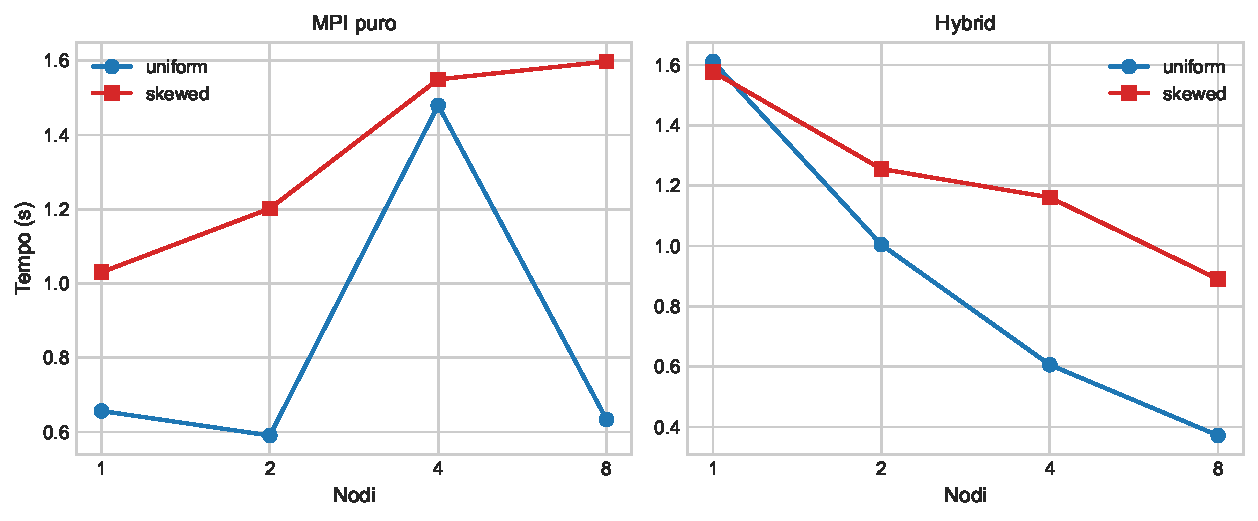
\includegraphics[width=\linewidth]{fig_skew.pdf}
  \caption{Total time under uniform vs.\ skewed input
    ($\rho=0.9$, 4 hot keys).}
  \label{fig:skew}
\end{figure}

%---------------------------------------------------------------
\section{Comparison with the Shared-Memory Versions}
%---------------------------------------------------------------
On a single node the pure-MPI run with 32 ranks completes in
\SI{0.66}{s} (speedup $6.9\times$ over the sequential M3 baseline),
while the hybrid with one rank and 32 threads takes \SI{1.61}{s}
($2.8\times$). The gap closes from two nodes onwards: hybrid takes
\SI{1.00}{s} at two nodes vs.\ \SI{0.59}{s} for MPI, and from four
nodes onwards hybrid is faster than pure MPI both in absolute
terms (\SI{0.61}{s} vs.\ \SI{1.48}{s}) and in worst-case
predictability. The cross-over is driven by the
\texttt{Alltoallv} cost: pure MPI keeps the local phases cheap by
splitting them across 32 ranks per node, but pays an
ever-increasing communication tax as the global rank count grows;
the hybrid amortises a small parallelisation overhead in the
local phases against a much cheaper collective.

Relative to Module~3's OpenMP loop variant the hybrid M4 binary
matches the multi-thread shared-memory result at one node (the
local pipeline is essentially the same with an added MPI no-op),
and from two nodes onwards extends the curve into the
distributed-memory regime, where M2 and M3 cannot follow at all.

%---------------------------------------------------------------
\section*{Conclusions}
%---------------------------------------------------------------
The distributed implementation preserves the algorithmic structure
of the previous modules and re-uses the M3 build/probe kernel
unchanged. Within the eight-node budget of the cluster the hybrid
pipeline reaches a $12.2\times$ speedup over the sequential M3
baseline on uniform input with $0.57$ weak-scaling efficiency,
beating the $7.7\times$/$0.20$ obtained by pure MPI. The
breakdown confirms that further speedup is communication-bound:
\texttt{Alltoallv} is the largest contribution to wall time in
every multi-node configuration. The hybrid variant pays a
non-trivial single-node cost for parallelising the local phases
with OpenMP, but it amortises that cost across nodes and is
preferable from two nodes onwards.

% ------------- Hybrid MPI+OpenMP addendum (1 extra page) -------
\onecolumn\newpage
\section*{Addendum: Hybrid MPI+OpenMP}
The hybrid configuration uses one MPI rank per node with
\texttt{OMP\_NUM\_THREADS=32}, \texttt{OMP\_PROC\_BIND=close} and
\texttt{OMP\_PLACES=cores}. \emph{Every} per-rank phase is
OpenMP-parallel: \emph{histogram\_local} and \emph{histogram\_post}
build per-thread private histograms and merge them at the end,
\emph{scatter\_local} and \emph{scatter\_post} reuse those
per-thread tables to derive per-thread offsets so writes never
collide on the same slot of the output buffer, and
\emph{join\_local} runs a \texttt{parallel for} with
\texttt{schedule(dynamic)} and a sum reduction. The static
scheduling on the scatter passes mirrors the histogram pass that
fed it, so the same input range is visited by the same thread in
both phases.

\paragraph{Effect on the single-node case.}
A first version of the hybrid parallelised only \emph{join\_local}
and left the other four local phases single-threaded. That
implementation took \SI{6.25}{s} on one node — slower than the
sequential M3 baseline — because the only rank had to scan all
\SI{150}{M} records through one CPU pipeline before reaching the
parallel join. Parallelising all local phases brings the one-node
hybrid down to \SI{1.61}{s}, a $3.9\times$ improvement, and is
what makes the multi-node curve of Figure~\ref{fig:strong}
monotonic. The takeaway is structural: in a hybrid pipeline the
sequential phase always becomes the bottleneck (Amdahl, lez.~10),
and parallelising the obvious hot loop is not enough.

\paragraph{Collective cost.}
Going from 256 ranks (pure MPI on 8 nodes) to 8 ranks (hybrid on
8 nodes) reduces the median \texttt{Alltoallv} time on uniform
input from \SI{0.53}{s} to \SI{0.18}{s}, a $3\times$ speedup with
the same total payload moved. \texttt{Allreduce} of the three
aggregates is consistently below a millisecond regardless of node
count because it sees only 1 to 8 participants. The collective
cost still dominates the wall time of the hybrid (around $44\%$
at four nodes and growing with $N$), which suggests that the next
optimisation to consider is communication--computation overlap:
posting the \texttt{Alltoallv} as a non-blocking
\texttt{MPI\_Ialltoallv} while the local build step starts on the
partitions that are already known to be local.

\paragraph{Rank-per-socket layout.}
The compute nodes have two NUMA domains; binding one rank per
socket (two ranks per node, 16 threads each) would let the local
join run entirely within one NUMA domain at the cost of doubling
the \texttt{Alltoallv} fan-out. Given that the local phases are
now parallel and the wall time is communication-bound, doubling
the rank count is unlikely to help; the experiment was not run
within the time budget.

\end{document}
